\documentclass[12pt]{article}
\usepackage{hyperref}
\usepackage{amsmath, amssymb, amsfonts}
\usepackage[margin=1.2cm]{geometry}
\usepackage{xcolor}
\usepackage{graphicx}
\usepackage{enumitem}
\parindent 0pt
\newcommand{\lb}{\\$\left|\rightarrow\right.$}
\newcommand{\enter}{\\\textcolor{white}{1}}
\ExplSyntaxOn
\NewDocumentCommand{\bo}{m}
 {
   \bold_commas:n { #1 }
 }
\cs_new:Npn \bold_commas:n #1
 {
   \seq_set_split:Nnn \l_tmpa_seq { , } { #1 }
   \seq_map_indexed_function:NN \l_tmpa_seq \__bold_commas_aux:nn
 }
\cs_new:Npn \__bold_commas_aux:nn #1 #2
 {
   \textbf{#2}
   \int_compare:nNnTF { #1 } < { \seq_count:N \l_tmpa_seq }
     { , }
     { }
 }
\ExplSyntaxOff

\title{Artificial Intelligence (CT653 / CT710)\\[0.4em]\large Detailed PYQ}
\author{}
\date{\today}

\begin{document}
\maketitle
\vspace{6cm}
\textbf{Notes}
\begin{itemize}[noitemsep]
  \item Questions from Tribhuvan University, IOE (2069--2081 BS), sorted by the CT710 syllabus.
  \item Regular exam = \bo{bold}, Back exam = regular font.
  \item BCT programme (CT653) = normal font, BEI programme (CT710) = \texttt{this monospace style}.
  \item So: \bo{72 Ash} = BCT Regular, 73 Ma = BCT Back, \bo{\texttt{79 Bh}} = BEI Regular, \texttt{81 Ba} = BEI Back.
  \item Months: Bh = Bhadra, Po = Poush, Ma = Magh, Ash = Ashwin, Ba = Baishakh, Ch = Chaitra.
  \item Keywords: (I) = Importance/Need/Significance, (+) = Advantage, (-) = Disadvantage, +Fig = Figure/Diagram, +Eg = Example, Vs = Compare/Differentiate.
\end{itemize}
\pagebreak
\tableofcontents
\pagebreak

%=======================================================================
\section{Introduction}
\begin{center}(7 Hours)\end{center}

  \subsection{Definition of AI, Agents and the Turing Test}
    \begin{enumerate}[topsep=0pt, noitemsep]
      \item Define AI. When is a machine said to have passed the Turing test? Give two examples of constraint satisfaction problem. \hfill [2+5+1] (\bo{70 Bh})
        \lb What is AI? Explain the Turing test and its importance in AI. \hfill [7] (69 Po)
        \lb What is the importance of Turing Test in AI? List applications of AI. \hfill [2+4+2] (75 Ba)
        \lb What is Turing test? How can it be used to measure intelligence of a machine? Explain. \hfill [2+5] (\bo{\texttt{79 Bh}})
        \lb Define intelligent agent. Explain the factors required to pass the Turing Test. \hfill [2+6] (\texttt{81 Ba})

      \item If the Turing Test is passed, does this show that computers exhibit intelligence? State your reasons. \hfill [7] (72 Ma, \bo{73 Bh})

      \item What is a rational agent? ``Systems that think like humans'' and ``systems that act like humans'' are part of AI --- justify with practical example. \hfill [1+6] (\bo{74 Bh})
        \lb Define AI and Intelligent agent. Differentiate between the different types of intelligent agent with examples. \hfill [2+6] (\bo{\texttt{80 Bh}})
        \lb What is an intelligent agent? What type of model does it work on? Explain PEAS for a Medical Diagnosis System. \hfill [2+2+3] (\texttt{80 Ba})

      \item Define AI. Differentiate between Natural (Human) Intelligence and Artificial Intelligence. Can AI replace humans? Justify. \hfill [1+3+4] (\bo{79 Ch})
    \end{enumerate}

  \subsection{Importance of AI}
  \subsection{AI and related fields}
  \subsection{Brief history of AI}
    \begin{enumerate}[topsep=0pt, noitemsep]
      \item What is AI? Discuss brief history of AI with chronological development. \hfill [2+6] (70 Ma)
        \lb What is AI? Discuss history of AI in brief. \hfill [2+5] (\bo{71 Bh})
    \end{enumerate}

  \subsection{Applications of AI}
    \begin{enumerate}[topsep=0pt, noitemsep]
      \item Discuss any two fields of your daily life where AI has been applied. \hfill [7] (\bo{69 Bh})
        \lb What is AI? Explain any two applications of AI in the real field. \hfill [7] (\bo{72 Ash})
        \lb Define AI. Describe the importance and practical application of AI. \hfill [6] (73 Ma)
    \end{enumerate}

  \subsection{Definition and importance of Knowledge and Learning}
    \begin{enumerate}[topsep=0pt, noitemsep]
      \item Distinguish between knowledge and learning. What does acting humanly refer to? Explain. Define well defined problems. \hfill [2+5+1] (71 Ma)

      \item ``Learning is an essential characteristic for intelligent agents.'' Justify this statement. Write about the role of learning with a suitable example. \hfill [4+4] (\bo{73 Bh})
    \end{enumerate}

\pagebreak
%=======================================================================
\section{Problem Solving}
\begin{center}(7 Hours)\end{center}

  \subsection{Defining problems as a state space search / Problem formulation}
    \begin{enumerate}[topsep=0pt, noitemsep]
      \item What are the steps of Problem solving? You are given three empty jugs: a 3-gallon, a 5-gallon and a 9-gallon, and a pump can fill water only in the 3-gallon jug. How do you get exactly 7 gallons in the 9-gallon jug? Formalize the problem, write production rules and draw the search tree. \hfill [2+1+2+3] (\bo{\texttt{79 Bh}})

      \item A farmer has a goat, a wolf and a cabbage on the west side of a river and wants to move everything to the east side. The boat holds the farmer and one other thing. The wolf eats the goat and the goat eats the cabbage if left alone. Formulate this puzzle as search and solve it (any method); draw the search tree and final solution. \hfill [8] (73 Ma)
    \end{enumerate}

  \subsection{Well-defined problems}
    \begin{enumerate}[topsep=0pt, noitemsep]
      \item What makes a problem ``Well Defined''? Explain with a sample example of a state-space search framework. \hfill [3+4] (\bo{71 Bh})
        \lb What is problem space? (asked with crypto-arithmetic below). \hfill [2] (Back)
    \end{enumerate}

  \subsection{Constraint Satisfaction Problem (crypto-arithmetic)}
    \begin{enumerate}[topsep=0pt, noitemsep]
      \item Solve the following crypto-arithmetic problem through constraint satisfaction, showing all steps.
        \lb LOGIC + LOGIC = PROLOG \hfill [7] (\bo{69 Bh}) [3+4] (72 Ma) [3+5] (\bo{79 Ch})
        \lb RIGHT + RIGHT = WRONG \hfill [7] (69 Po)
        \lb WRONG + WRONG = RIGHT \hfill [5+3] (\bo{70 Bh})
        \lb ONE + ONE + TWO = FOUR \hfill [7] (71 Ma, \bo{73 Bh})
        \lb SEND + MORE = MONEY \hfill [1+6] (\bo{72 Ash})
        \lb SWIM + WEAR = RELAX \hfill [1+6] (\bo{74 Bh})
        \lb BASE + BALL = GAMES (What is problem space?) \hfill [2+6] (75 Ba)
        \lb TEN + TEN + FORTY = SIXTY \hfill [2+6] (\bo{\texttt{80 Bh}})
        \lb LOVE + LOVE = HATE (What is a well-defined problem?) \hfill [2+6] (\texttt{81 Ba})
        \lb EAT + THAT = APPLE \hfill [2+6] (\texttt{80 Ba})
    \end{enumerate}

  \subsection{Game playing, Production systems}
    \begin{enumerate}[topsep=0pt, noitemsep]
      \item Why is searching necessary in AI? Explain the role of production system with a suitable example. \hfill [2+6] (70 Ma)
    \end{enumerate}

\pagebreak
%=======================================================================
\section{Search Techniques}
\begin{center}(9 Hours)\end{center}

  \subsection{Necessity of searching}
    \begin{enumerate}[topsep=0pt, noitemsep]
      \item Explain the necessity of searching techniques in AI. \hfill [various]
        \lb Searching is an important part of AI, justify it. Explain any two types of blind search and compare them in terms of space and time complexity. \hfill [2+7] (72 Ma)
        \lb Why is searching important in problem solving? What are the drawbacks of greedy best-first search and how does A* solve it? Explain with example. \hfill [2+7] (\bo{74 Bh})
    \end{enumerate}

  \subsection{Uninformed search --- DFS, BFS, depth limit search, comparison}
    \begin{enumerate}[topsep=0pt, noitemsep]
      \item What is a searching? Explain Breadth First Search and Depth First Search and compare their performance criteria. \hfill [9] (\bo{72 Ash})
        \lb What is blind search? Explain depth first search with an example and compare it with breadth first search. \hfill [9] (69 Po)
        \lb Differentiate between informed and blind search. How is depth first search different from breadth first search? Compare with evaluation parameters. \hfill [4+4] (\bo{70 Bh})
        \lb What is horn clause? Differentiate between Depth First Search and Breadth First Search. \hfill [1+7] (70 Ma)
        \lb Explain the necessity of searching techniques in AI. Differentiate between BFS and DFS with their performance criteria. \hfill [4+5] (\bo{73 Bh}) [7] (\bo{\texttt{79 Bh}})

      \item What is the advantage of depth limit search? Compare it with other search strategies. \hfill [4+4] (\bo{71 Bh})
    \end{enumerate}

  \subsection{Informed search --- hill climbing, best first, greedy, A*}
    \begin{enumerate}[topsep=0pt, noitemsep]
      \item Discuss the hill-climbing search algorithm along with the problems associated with it and their solutions. \hfill [9] (\bo{69 Bh})
        \lb \dots Why is simulated annealing important? \hfill [6+2] (75 Ba)
        \lb What are the problems associated with hill climbing search? Explain how simulated annealing overcomes them. \hfill [3+5] (\texttt{80 Ba})
        \lb Compare informed and uninformed search techniques. What strategies address the issue of local maxima in Hill Climbing Search? \hfill [4+4] (\texttt{81 Ba})

      \item Devise an example to show how A* algorithm uses path cost and heuristic cost to generate the best solution. \hfill [8] (73 Ma)
        \lb Why is searching important in problem solving? Drawbacks of greedy best-first search and how A* solves it, with example. \hfill [2+7] (\bo{74 Bh})
    \end{enumerate}

  \subsection{Adversarial search --- minimax, alpha-beta}
    \begin{enumerate}[topsep=0pt, noitemsep]
      \item How is informed search different from uninformed search? Explain the min-max algorithm with a suitable example, and discuss how alpha-beta is different from the min-max algorithm. \hfill [2+4+3] (71 Ma)

      \item What is minmax search? Apply minmax search along with alpha-beta pruning for the following tree (max node at top). \hfill [2+6] (\bo{79 Ch})\\
      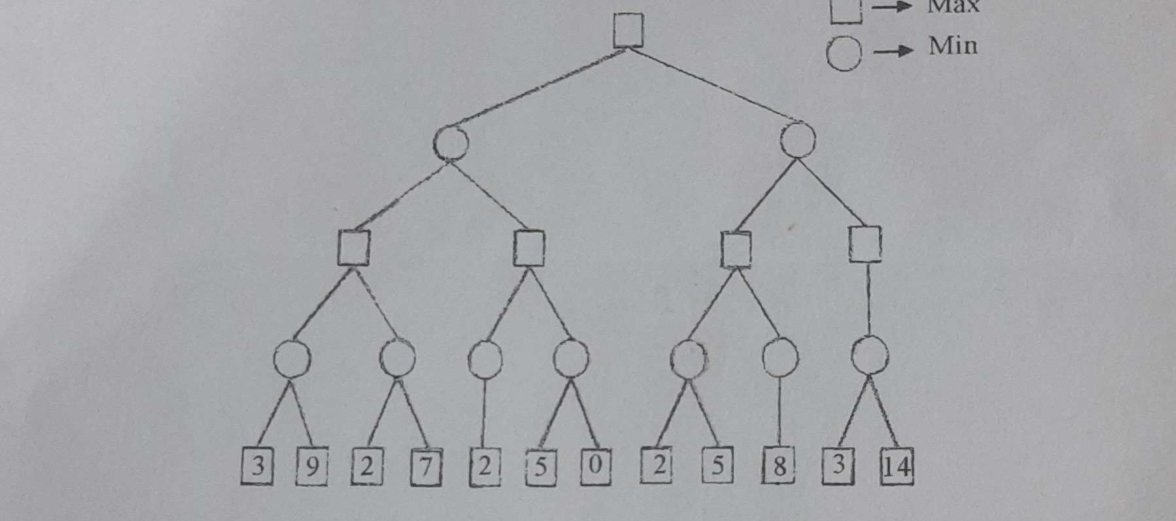
\includegraphics[width=5in]{images/ai_79ch_minmax.png}

      \item How is searching done in adversarial search? How does A* search overcome the problem associated with Greedy Search? Explain with example. \hfill [2+6] (\bo{\texttt{80 Bh}})
    \end{enumerate}

\pagebreak
%=======================================================================
\section{Knowledge Representation, Inference and Reasoning}
\begin{center}(4 Hours)\end{center}

  \subsection{Formal logic and Conjunctive Normal Form (CNF)}
    \begin{enumerate}[topsep=0pt, noitemsep]
      \item Explain all the steps involved in conversion to conjunctive normal form (CNF) with a suitable example. \hfill [10] (69 Po) [8] (\bo{70 Bh})
        \lb Why is CNF required? Explain all the steps used to convert a quantified statement, with example. \hfill [2+6] (75 Ba)
        \lb Why is CNF necessary? Represent ``Everyone who loves all animals is loved by someone'' in FOPL and convert it to CNF. \hfill [2+6] (\bo{79 Ch})
    \end{enumerate}

  \subsection{Propositional / predicate logic, FOPL, Horn clauses, Skolemization}
    \begin{enumerate}[topsep=0pt, noitemsep]
      \item Why do we need FOPL? State any three rules of inference. How can we make a machine with learning capacity? \hfill [2+3+3] (71 Ma)

      \item Define skolemization with example. \hfill [2] (\texttt{81 Ba}) \quad (also short note, \bo{69 Bh})
    \end{enumerate}

  \subsection{Rules of inference, unification, resolution refutation, deduction}
    \begin{enumerate}[topsep=0pt, noitemsep]
      \item Prove the goal using FOPL/resolution refutation from the given premises:
        \lb Every American who sells weapons to hostile nations is a criminal. The country Abc is enemy of America. All of the missiles in Abc were sold by John. John is an American. Prove John is a criminal. \hfill [10] (\bo{69 Bh})
        \lb Every American who sells weapons to hostile nations is a criminal. The country XYZ is enemy of America. All of its missiles in XYZ were sold by Donald, who is an American. Prove that Donald is a criminal using FOPL based resolution refutation. \hfill [8] (Back, \bo{75 Ba})
        \lb All oversmart persons are stupid. Children of oversmart persons are naughty. Ram is children of Hari. Hari is oversmart. Show that Ram is naughty using FOPL based resolution. \hfill [8] (\bo{70 Bh})
        \lb If X is on the top of Y, Y supports X. If X is above Y and they are touching each other, X is on the top of Y. A cup is above a book. A cup is touching a book. Show that supports(book, cup) is true. \hfill [8] (\bo{71 Bh})
        \lb Assume the following facts: John likes all kinds of food; apples are food; chicken is food; anything anyone eats and isn't killed by is food; Bill eats peanuts and is still alive; Sue eats everything Bill eats. Prove that John likes peanuts using resolution refutation. \hfill [7] (\bo{72 Ash}) [8] (\bo{74 Bh})
        \lb Assume the following facts: a) Sita likes all kinds of food; b) Momo and Burger are food; c) anything anyone eats and isn't killed by is food; d) Bill eats mushroom and is still alive; e) Sue eats everything Bill eats. Prove that ``Sita likes mushroom'' using resolution refutation method. \hfill [8] (\texttt{80 Ba})
        \lb Using resolution, solve the following statements: All pompeian are Romans. All Romans were either loyal to Caesor or hated him. Everyone is loyal to someone. People only try to assassinate rulers they not loyal to. Marcus tried to assassinate Caesor. Marcus was pompeian. Find, did Marcus Caesor? \hfill [7] (72 Ma)
        \lb Assume the following facts: i) horses, cows, pigs are mammals; ii) an offspring of a horse is a horse; iii) Bluebeard is a horse; iv) Bluebeard is Charlie's parent; v) offspring and parent are inverse relations; vi) every mammal has a parent. Prove Charlie is a horse using resolution refutation. \hfill [8] (\bo{73 Bh})
        \lb Prove that ``Charlie is a mammal'' with given propositions: a) cows, pigs and horses are mammal; b) the child of horse is a horse; c) Bluebeard is a horse; d) Bluebeard is Charlie's father; e) child and father are inverse relation; f) every mammal has a father. \hfill [8] (\bo{\texttt{79 Bh}})
        \lb Consider the following axioms: i) anyone whom Mary loves is a football star; ii) any student who does not pass does not play; iii) John is a student; iv) any student who does not study does not pass; v) anyone who does not play is not a football star. Prove that ``If John does not study, then Mary does not love John'' using resolution by refutation. \hfill [10] (73 Ma)
        \lb Assume the following facts: i) Ram likes all kinds of food; ii) apples and vegetables are food; iii) anything anyone eats and not killed is food; iv) Anil eats peanuts and is still alive; v) Ram eats everything that Anil eats. Prove that ``Ram likes peanuts'' using resolution refutation. \hfill [8] (\bo{\texttt{80 Bh}})
        \lb Define skolemization with example. Consider the following axioms: a) anyone passing his engineering exams and winning the lottery is happy; b) anyone who studies or is lucky can pass all his exams; c) Sneha did not study but she is lucky; d) anyone who is lucky wins the lottery. Using resolution refutation, prove that Sneha is happy. \hfill [2+6] (\texttt{81 Ba})

      \item What is rule based reasoning? Explain Backward Chaining with a suitable example. \hfill [7] (72 Ma)
        \lb Explain backward chaining with a suitable example and compare with forward chaining. \hfill [4+4] (70 Ma)
        \lb Explain Backward Chaining with a suitable example. \hfill [7] (\bo{71 Bh})

      \item What is knowledge, representation and reasoning? Describe forward chaining with a practical example. \hfill [2+5] (\bo{72 Ash})
        \lb Differentiate between forward and backward chaining using a suitable example. \hfill [4] (\bo{74 Bh}) [7] (\bo{\texttt{79 Bh}})
    \end{enumerate}

  \subsection{Statistical reasoning --- Probability, Bayes' theorem, causal/belief networks}
    \begin{enumerate}[topsep=0pt, noitemsep]
      \item What is causal network? Explain reasoning in belief network with suitable example. \hfill [2+5] (71 Ma)
        \lb What is belief network? How reasoning is done in this network? \hfill [2+6] (\bo{79 Ch})

      \item What is causal net? How does Bayes' Theorem calculate the probability in a causal net? Explain with example calculation. \hfill [7] (\bo{73 Bh})
        \lb What is neural network? Describe its types. A doctor knows that the disease meningitis causes the patient to have a stiff neck 50\% of the time. The doctor also knows that the probability that a patient has meningitis is 1/50,000, and the probability that any patient has a stiff neck is 1/20. Find the probability that a patient with a stiff neck has meningitis? \hfill [3+5] (71 Ma)
        \lb A doctor is called to see a sick child. The doctor has prior information that 90\% of sick children in that neighborhood have the flu, while the other 10\% are sick with measles. Let F stand for an event of a child being sick with Flu and M stand for an event of a child being sick with measles. Assume for simplicity that there no other maladies in that neighborhood. A well-known (and common) symptom of measles is a rash and has probability of 0.95. However, very occasionally, children with flu also develop rash and has probability of 0.08. Upon examining the child, the doctor finds a rash. What is the probability that the child has measles? \hfill [8] (73 Ma)
        \lb What is prior probability and posterior probability? A doctor knows that the disease meningitis causes a patient to have a stiff neck, say, 80\% of the time. The doctor also knows some unconditional facts: the prior probability that any patient has meningitis is 1/50000, and the prior probability that any patient has a stiff neck is 1\%. Determine the probability of meningitis when a patient has a stiff neck. \hfill [2+6] (\texttt{81 Ba})

      \item What do you understand by Bayesian Network? In a County, 51\% of the adults are males and the other 49\% are females. One adult is randomly selected for a survey involving credit card usage. i) Find the prior probability that the selected person is a male. ii) It is later learned that the selected survey subject was smoking a cigar. Also, 9.5\% of males smoke cigars, whereas 1.7\% of females smoke cigars (based on data from the Substance Abuse and Mental Health Services Administration). Use this additional information to find the probability that the selected subject is a male. \hfill [2+6] (\bo{\texttt{80 Bh}})
        \lb What is Bayesian network? Describe with an appropriate example. How inference can be done using this network? \hfill [5+3] (\texttt{80 Ba})
    \end{enumerate}

\pagebreak
%=======================================================================
\section{Structured Knowledge Representation}
\begin{center}(4 Hours)\end{center}

  \subsection{Approaches and Issues in Knowledge Representation}
    \begin{enumerate}[topsep=0pt, noitemsep]
      \item What are the different knowledge representation models? Discuss semantic nets with an example. \hfill [7] (\bo{69 Bh}) [2+5] (\texttt{80 Ba})

      \item How is a knowledge representation evaluated? Explain semantic net and frame representation with examples. \hfill [3+5] (\bo{\texttt{80 Bh}})
        \lb List the issues need to be consider in Knowledge Representation techniques. Convert the given sentences into a Semantic Network (sentence list under \textit{Semantic nets} below). \hfill [2+6] (\bo{\texttt{79 Bh}})
    \end{enumerate}

  \subsection{Semantic nets}
    \begin{enumerate}[topsep=0pt, noitemsep]
      \item What is semantic net? Explain with a suitable example. \hfill [8] (\bo{70 Bh})

      \item Convert the given sentences into a Semantic Network.
        \lb What are Frames and Semantic Net? Convert the given sentences in semantic Net: i) A person is a mammal. ii) Sakti Gauchan is a person. iii) Person has nose. iv) Sakti Gauchan is in Nepalese team. v) Uniform color of Sakti Gauchan is Red/Blue. \hfill [7] (72 Ma)
        \lb Convert given sentences into Semantic Network: i) The height of the adult male is 5.10. ii) Baseball player is an adult male. iii) Adult male is a person. iv) Batting average of Baseball players is 0.252. v) Pee-wee-Reese is a Fielder. vi) Fielder is Baseball player. vii) Team of Pee-wee-Reese is Brooklyn Dodger. \hfill [7] (\bo{73 Bh})
        \lb What is semantic network? Convert the following sentences into semantic network: i) The avg height of an adult is 5'6''. ii) Cricket player is an adult male. iii) Adult male is a person. iv) Batting average of a cricket player is 37.59. v) Rohit Paudel is a Fielder. vi) Fielder is a cricket player. vii) Team of Rohit Paudel is Nepal. \hfill [2+6] (\bo{79 Ch})
        \lb List the issues need to be consider in Knowledge Representation techniques. Convert given sentences into Semantic Network: a) Tom is a cat. b) Tom fights with rat. c) Tom is owned by Ram. d) Tom is black in color. e) Cats like milk. f) Rats like cheese. g) The cat sat on the bed. h) A cat is a mammal. i) A Rat is an animal. j) All mammals are animals. k) Every mammal gives birth a baby. \hfill [2+6] (\bo{\texttt{79 Bh}})

      \item Give an example of learning by analogy. How can knowledge be represented using a semantic network? Explain with example. \hfill [1+7] (\bo{71 Bh})
    \end{enumerate}

  \subsection{Frames}
    \begin{enumerate}[topsep=0pt, noitemsep]
      \item What is a frame? Explain with a suitable example. \hfill [7] (69 Po)
        \lb What is Frame? How is it different from semantic net in knowledge representation? \hfill [7] (\bo{74 Bh})

      \item What are semantic nets and frames? How are frames useful in semantic nets? \hfill [7] (\bo{72 Ash})
        \lb What are Frames and Semantic Net? Convert the given sentences into semantic net. \hfill [7] (72 Ma)
        \lb Explain Frames and Semantic Net with examples. List their advantages and limitations. \hfill [4+4] (73 Ma)

      \item Why are semantic networks and frames important in AI? Provide examples of both with FOPL statements. \hfill [2+6] (75 Ba)
        \lb Compare semantic net and frame. How do you convert a semantic net into a frame? Explain with example. \hfill [3+5] (\texttt{81 Ba})
    \end{enumerate}

  \subsection{Conceptual dependencies and scripts}
    \begin{enumerate}[topsep=0pt, noitemsep]
      \item What is conceptual dependency? Explain some of the common primitives used in conceptual dependency. \hfill [2+5] (\bo{71 Bh})
    \end{enumerate}

\pagebreak
%=======================================================================
\section{Machine Learning}
\begin{center}(6 Hours)\end{center}

  \subsection{Concepts of learning}
    \begin{enumerate}[topsep=0pt, noitemsep]
      \item What are the different methods for learning? (asked with genetic algorithm / flowchart). \hfill [3+5] (\texttt{81 Ba})
    \end{enumerate}

  \subsection{Learning by analogy, Inductive learning, Explanation based learning}
    \begin{enumerate}[topsep=0pt, noitemsep]
      \item Give an example of learning by analogy (with semantic network). \hfill [1+7] (\bo{71 Bh})

      \item Define inductive learning. Explain in detail the ID3 process with a suitable example. \hfill [2+6] (\bo{74 Bh})
    \end{enumerate}

  \subsection{Genetic algorithm}
    \begin{enumerate}[topsep=0pt, noitemsep]
      \item What is genetic algorithm (GA)? Explain the operators of GA along with its importance. \hfill [10] (69 Po)
        \lb What is machine learning? Explain GA along with different operators of genetic algorithm. \hfill [2+8] (71 Ma)
        \lb What is machine learning? Explain GA along with GA operators. List some areas where GA can be applied. \hfill [2+6+2] (72 Ma)
        \lb What is a genetic algorithm? Explain all steps in GA with block diagram and operators. \hfill [8] (75 Ba)
        \lb What is evolutionary computing? List the steps in genetic algorithm with an example. \hfill [2+6] (\bo{79 Ch})
        \lb Discuss the steps involved in genetic algorithm with example. \hfill [8] (\texttt{80 Ba})
        \lb What are the different methods for learning? Explain the steps in GA with a flowchart and justify why mutation is important. \hfill [3+5] (\texttt{81 Ba})

      \item What is machine vision? Discuss the algorithm of Genetic Algorithm. \hfill [2+6] (\bo{70 Bh})

      \item Justify that the study of gene is one important part of AI. List the steps involved in genetic algorithm with an example. \hfill [4+4] (\bo{74 Bh})
    \end{enumerate}

  \subsection{Fuzzy learning}
    \begin{enumerate}[topsep=0pt, noitemsep]
      \item What is fuzzy learning? Explain with a practical example. \hfill [4] (\bo{69 Bh})

      \item What is Machine Learning? What is Fuzzy Logic? Explain Fuzzy Inference with a suitable example. \hfill [2+6] (70 Ma)
        \lb What is Fuzzy Logic and why is it important? Explain the Mamdani Fuzzy Inference Method with example. \hfill [3+7] (73 Ma)

      \item Explain all the steps in Fuzzy Learning with a block diagram and an example. \hfill [8] (\bo{\texttt{80 Bh}})
        \lb What do you mean by membership of an element in a fuzzy set? Explain the steps involved in Fuzzy Learning with a suitable example. \hfill [2+6] (\bo{\texttt{79 Bh}})
    \end{enumerate}

  \subsection{Boltzmann Machines}
    \begin{enumerate}[topsep=0pt, noitemsep]
      \item Define Boltzmann Machine. How can knowledge be represented using a semantic network? Explain with example. \hfill [1+7] (70 Ma)
        \lb What is machine learning? Explain in detail about Boltzmann machines with suitable algorithm and explanations. \hfill [2+8] (\bo{72 Ash})
    \end{enumerate}

\pagebreak
%=======================================================================
\section{Applications of AI}
\begin{center}(14 Hours)\end{center}

  \subsection{Neural Networks (structure, Adaline, Perceptron, MLP/Back-propagation, Hopfield, Kohonen)}
    \begin{enumerate}[topsep=0pt, noitemsep]
      \item What is a neural network? Explain the back-propagation algorithm (learning). \hfill [4+4] (\bo{70 Bh})
        \lb What is a neural network? Explain the back propagation algorithms and perceptron. \hfill [2+4+4] (\bo{72 Ash})
        \lb What is the role of perceptron in neural network? Explain the back-propagation algorithm. \hfill [3+5] (71 Ma)
        \lb Describe the mathematical model of a neural network. What does it mean to train a neural network? Write an algorithm for its learning. \hfill [2+2+4] (\bo{\texttt{80 Bh}})
        \lb Define ANN. How can non-linearity be modelled through this ANN? Explain with example. \hfill [1+7] (\bo{\texttt{79 Bh}})

      \item What is a neural network? Differentiate between supervised and unsupervised learning. \hfill [6] (69 Po)

      \item What is Artificial Neural Network (ANN)? Compare ANN with the human brain and its functioning principle. \hfill [3+5] (\bo{71 Bh})

      \item What do you understand by a perceptron? How can we design a neural network that acts as an OR gate? \hfill [2+7] (72 Ma)
        \lb What do you understand by Perception? How can we design a neural network that acts as an XOR gate? \hfill [1+7] (73 Ma)
        \lb What is perceptron? When do we need the back propagation algorithm? Explain with an example. \hfill [2+6] (\bo{79 Ch})

      \item What is a McCulloch/Pitts neural network? Explain it with reference to AND gate and justify that it cannot be applied to Exclusive OR gate. \hfill [8] (75 Ba)

      \item Define Hebbian learning. Use the Hebbian learning algorithm to construct a Hebbian Network which performs the AND function. \hfill [3+7] (\bo{73 Bh})
        \lb What is perception? Construct a Hebbian Network that performs like AND Gate. \hfill [2+6] (\texttt{81 Ba})

      \item What is a Hopfield Network? Explain all the steps involved in the Hopfield Network with a suitable example. \hfill [8] (\bo{69 Bh})

      \item What is Self-Organizing Map (SOM)? Explain all the steps involved in SOM with a suitable example. \hfill [2+5] (\bo{74 Bh}) \quad (short note: \bo{\texttt{80 Bh}}, \bo{\texttt{79 Bh}})
    \end{enumerate}

  \subsection{Expert System (architecture, knowledge acquisition, KR, development)}
    \begin{enumerate}[topsep=0pt, noitemsep]
      \item Explain different steps of expert system development with an example. \hfill [8] (\bo{69 Bh})
        \lb What is an expert system? Explain the steps of expert system development. \hfill [4+4] (\bo{70 Bh})
        \lb What are the applications of Expert System? Describe the development stages of Expert System briefly. \hfill [2+6] (\bo{73 Bh})
        \lb List the importance of expert system in real life. Draw the block diagram of expert system architecture and explain all blocks. \hfill [2+6] (75 Ba)
        \lb What is expert system? Create a scenario where we require an expert system. List the steps of creating this system. \hfill [2+6] (\bo{79 Ch})

      \item What is an expert system? Explain the general architecture of an expert system. \hfill [8] (69 Po) [2+4] (71 Ma)
        \lb What are the major characteristics of an expert system? Explain with example. Explain a general approach for developing an expert system with a block diagram. \hfill [2+5] (\texttt{80 Ba})
        \lb What is expert system? Explain how inference is performed in an expert system. \hfill [3+5] (\texttt{81 Ba})

      \item Differentiate between declarative and procedural knowledge. Explain the architecture of an expert system (with practical uses). \hfill [2+6] (70 Ma) [3+6] (72 Ma) [3+5] (73 Ma)

      \item What is an expert system? Explain its advantages and disadvantages. \hfill [8] (\bo{72 Ash})

      \item Define knowledge acquisition with example. Explain the architecture of expert system. \hfill [2+6] (\bo{71 Bh})
        \lb How is knowledge acquisition performed in an expert system? Explain one real expert system example with proper architecture. \hfill [2+5] (\bo{74 Bh})
    \end{enumerate}

  \subsection{Natural Language Processing and Machine Vision}
    \begin{enumerate}[topsep=0pt, noitemsep]
      \item What is natural language processing? Explain it. \hfill [6] (\bo{69 Bh})
        \lb What is NLP? Explain the different steps of NLP. \hfill [8] (69 Po) [2+4] (73 Ma) [3+5] (\bo{79 Ch})
        \lb Justify that NLP is one of the important parts of AI. Explain the steps involved in NLP. \hfill [8] (75 Ba)
        \lb Explain the different steps involved in NLP with a suitable block diagram and examples. \hfill [8] (72 Ma)
        \lb Define NLU and NLG. List the different steps involved in NLP with suitable examples. \hfill [2+7] (\bo{73 Bh})

      \item Define machine translation in NLP. Explain the challenges of machine translation. \hfill [1+7] (\bo{70 Bh})
        \lb What is NLP? Discuss the different issues related to NLP with example. \hfill [2+6] (70 Ma)

      \item What is NLP? Explain the syntactic, semantic and pragmatic analysis of NLP. \hfill [2+2+2+2] (71 Ma)

      \item What are the problems associated with NLP? How is syntactic and semantic analysis done during NLP? Explain with example. \hfill [3+5] (\bo{\texttt{80 Bh}}) [2+5] (\texttt{80 Ba})
        \lb List the challenges faced by NLP. Why do you think machine vision is important in AI? Explain with example. \hfill [2+5] (\bo{\texttt{79 Bh}})

      \item How does machine vision help in Artificial Intelligence? Explain how the back propagation algorithm helps in machine learning. \hfill [3+5] (71 Ma)

      \item Short notes: Machine Vision / Computer Vision; Human Brain versus Neural Network; Skolemization; Horn clause; Perceptron; Supervised Vs Unsupervised learning; Back Propagation Algorithm; Fuzzy Logic; A* Search; Hill climbing algorithm. \hfill [various] (\bo{69 Bh}, 69 Po, \bo{74 Bh}, \texttt{80 Ba}, \texttt{81 Ba}, \bo{\texttt{79 Bh}})
    \end{enumerate}

\end{document}
